\documentclass[../../main]{subfiles}
\begin{document}
\label{ss:overall-system-architecture}
\subsection{Overall system architecture}
The system is divided in three main part:
    \begin{itemize}
        \item A Client;
        \item A Server;
        \item A Database.
    \end{itemize}

A overall picture describing the architecture is avaible at \hyperref[fig:system_architecture]{System architecture}.

\paragraph*{Authentication}
We want to use a mechanism that can generate an unique token starting from user data and store it in our database. ù
We'll use in the next APIs to check if the user from the request and the token provided in the Headers match.

\paragraph*{RESTful APIs}
The clients and the server communicate via RESTful APIs. We thought to implement a collection of APIs for each relevant part of data:

\begin{itemize}
    \item Points of Interest \textbf{'/points-of-interest'};
    \item Live Events \textbf{'/live-events'};
    \item Friends \textbf{'/friends'};
    \item Recommendation \textbf{'/recommendation'};

    \item Authentication \textbf{'/user-data'};

\end{itemize}
    \begin{figure}[h]
        \centering
        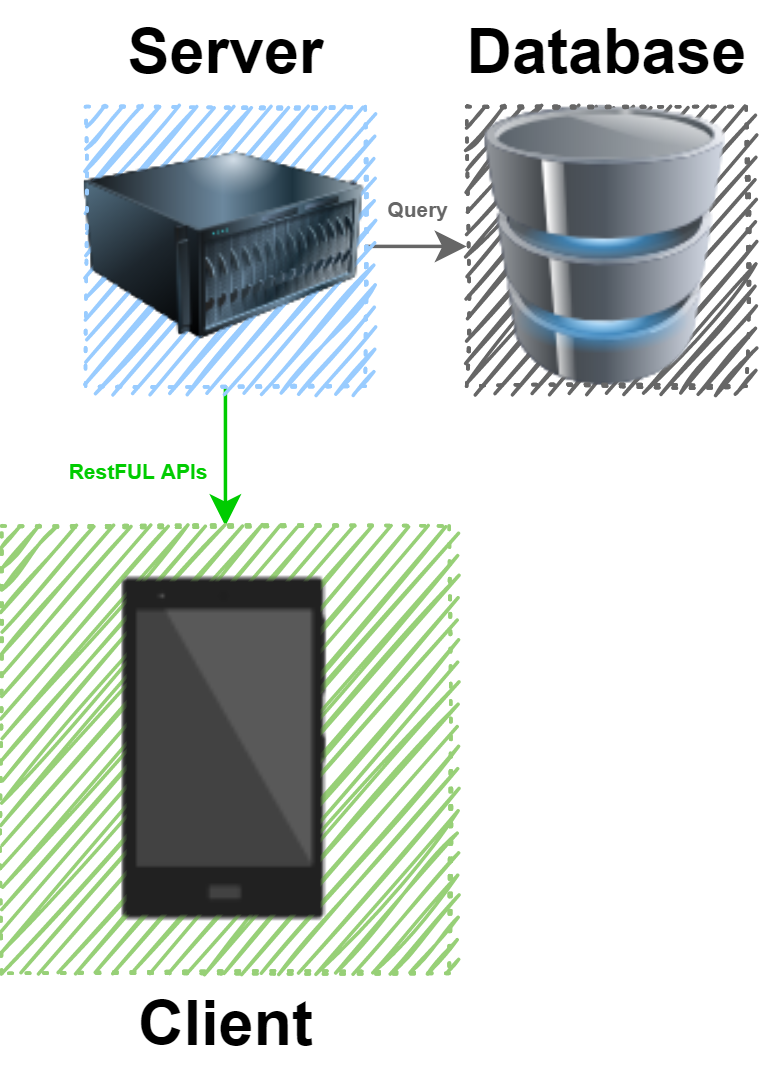
\includegraphics[width=100mm,height=130mm]{images/simple.png}
        \caption{Design of System Architecture}\label{fig:simple_system_architecture}
    \end{figure}

\paragraph*{Server}
The server is used to handle the communication with:
\begin{itemize}
    \item Database;
    \item Client;
    \item Prediction Model;
\end{itemize}
The server retrieves and manipulate, on request of the user, data from the \textbf{Database}, 
asks a recommendation to the model and sends the data that the client asked via RESTful APIs.
\end{document}